%\begin{figure}[!ht]
%\begin{centering}
%
%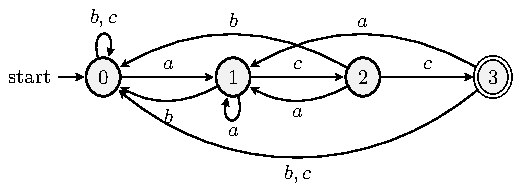
\includegraphics[width=0.35\textwidth]{./chapters/figures/forecasting/dfasr.pdf}
%\label{fig:dfa_adc}
%
%\hfill
%
%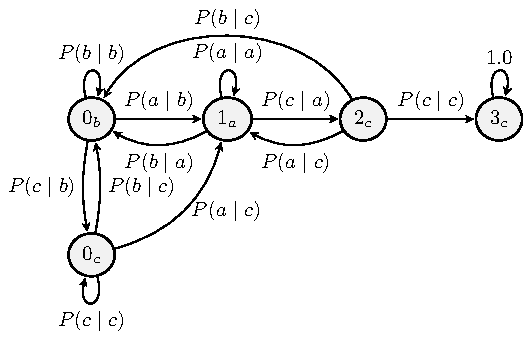
\includegraphics[width=0.35\textwidth]{./chapters/figures/forecasting/pmcr1.pdf}
%\label{fig:mc_adc}
%
%%\hfill
%\caption{DFA and PMC for $\mathcal{P}=a ; c ; c$,  $\Sigma=\{a,b,c\}$, and order $m=1$.}
%\label{fig:dfa_mc}
%\end{centering}
%\end{figure}

\begin{figure}[!h]
	\begin{centering}
		
	
			
			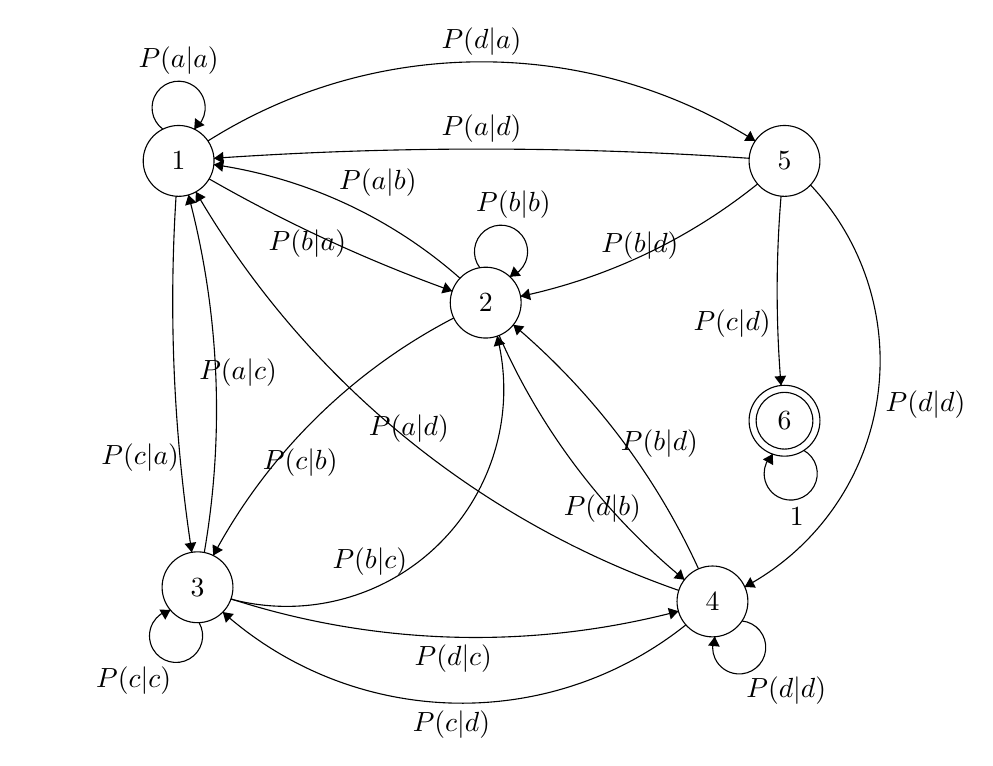
\begin{tikzpicture}[scale=.15]
			\tikzstyle{every node}+=[inner sep=0pt]
			\draw [black] (4.6,-12.2) circle (3);
			\draw (4.6,-12.2) node {$1$};
			\draw [black] (30.6,-24.2) circle (3);
			\draw (30.6,-24.2) node {$2$};
			\draw [black] (6.2,-48.3) circle (3);
			\draw (6.2,-48.3) node {$3$};
			\draw [black] (49.8,-49.5) circle (3);
			\draw (49.8,-49.5) node {$4$};
			\draw [black] (55.9,-12.2) circle (3);
			\draw (55.9,-12.2) node {$5$};
			\draw [black] (55.9,-34.2) circle (3);
			\draw (55.9,-34.2) node {$6$};
			\draw [black] (55.9,-34.2) circle (2.4);
			\draw [black] (3.277,-9.52) arc (234:-54:2.25);
			\draw (4.6,-4.95) node [above] {$P(a|a)$};
			\fill [black] (5.92,-9.52) -- (6.8,-9.17) -- (5.99,-8.58);
			\draw [black] (30.106,-21.253) arc (217.25487:-70.74513:2.25);
			\draw (32.95,-17.1) node [above] {$P(b|b)$};
			\fill [black] (32.64,-22.01) -- (33.58,-21.93) -- (32.97,-21.13);
			\draw [black] (6.328,-51.286) arc (30.18097:-257.81903:2.25);
			\draw (0.79,-55) node [below] {$P(c|c)$};
			\fill [black] (3.91,-50.22) -- (2.97,-50.19) -- (3.47,-51.05);
			\draw [black] (5.714,-45.34) arc (-171.29151:-183.63296:140.372);
			\fill [black] (5.71,-45.34) -- (6.09,-44.47) -- (5.1,-44.62);
			\draw (4.67,-37.32) node [left] {$\mbox{ }\mbox{ }\mbox{ }\mbox{ }\mbox{ }\mbox{ }\mbox{ }\mbox{ }P(c|a)$};
			\draw [black] (7.079,-10.512) arc (122.2697:57.7303:43.399);
			\fill [black] (53.42,-10.51) -- (53.01,-9.66) -- (52.48,-10.51);
			\draw (30.25,-3.31) node [above] {$P(d|a)$};
			\draw [black] (7.583,-12.513) arc (81.8726:48.57712:40.066);
			\fill [black] (7.58,-12.51) -- (8.3,-13.12) -- (8.45,-12.13);
			\draw (21.47,-15.28) node [above] {$P(a|b)$};
			\draw [black] (7.532,-45.612) arc (151.86818:117.42301:48.336);
			\fill [black] (7.53,-45.61) -- (8.35,-45.14) -- (7.47,-44.67);
			\draw (14.9,-36.53) node [below] {$P(c|b)$};
			\draw [black] (47.431,-47.66) arc (-129.36992:-156.24084:55.875);
			\fill [black] (47.43,-47.66) -- (47.13,-46.77) -- (46.5,-47.54);
			\draw (43.79,-41.65) node [left] {$\mbox{ }\mbox{ }P(d|b)$};
			\draw [black] (46.917,-50.329) arc (-75.2387:-107.9144:67.363);
			\fill [black] (46.92,-50.33) -- (46.02,-50.05) -- (46.27,-51.02);
			\draw (27.86,-53.1) node [below] {$P(d|c)$};
			\draw [black] (5.432,-15.082) arc (14.88666:-9.81113:70.847);
			\fill [black] (5.43,-15.08) -- (5.15,-15.98) -- (6.12,-15.73);
			\draw (6.31,-30.13) node [right] {$P(a|c)$};
			\draw [black] (27.764,-23.221) arc (-109.71785:-119.83243:128.561);
			\fill [black] (27.76,-23.22) -- (27.18,-22.48) -- (26.84,-23.42);
			\draw (15.5,-18.0) node [below] {$P(b|a)$};
			\draw [black] (31.568,-27.036) arc (14.17669:-104.88549:18.382);
			\fill [black] (31.57,-27.04) -- (31.28,-27.93) -- (32.25,-27.69);
			\draw (24,-46.09) node [left] {$P(b|c)$};
			\draw [black] (7.592,-11.979) arc (93.95767:86.04233:328.286);
			\fill [black] (7.59,-11.98) -- (8.42,-12.42) -- (8.36,-11.43);
			\draw (30.25,-10.7) node [above] {$P(a|d)$};
			\draw [black] (53.622,-14.151) arc (-51.2137:-78.03555:47.886);
			\fill [black] (33.55,-23.67) -- (34.44,-23.99) -- (34.23,-23.02);
			\draw (46.97,-20.61) node [above left] {$P(b|d)$};
			\draw [black] (55.607,-31.214) arc (-175.27936:-184.72064:97.384);
			\fill [black] (55.61,-31.21) -- (56.04,-30.38) -- (55.04,-30.46);
			\draw (54.78,-27.2) node [above left] {$P(c|d)$};
			\draw [black] (58.099,-14.237) arc (43.2333:-61.80904:21.727);
			\fill [black] (52.53,-48.27) -- (53.47,-48.33) -- (53,-47.45);
			\draw (64.42,-32.85) node [right] {$P(d|d)$};
			\draw [black] (52.291,-51.151) arc (84.18903:-203.81097:2.25);
			\draw (56.05,-55.84) node [below] {$P(d|d)$};
			\fill [black] (50,-52.48) -- (49.43,-53.23) -- (50.42,-53.33);
			\draw [black] (47.55,-51.483) arc (-51.43786:-131.71524:30.426);
			\fill [black] (8.34,-50.4) -- (8.6,-51.31) -- (9.27,-50.56);
			\draw (27.7,-58.68) node [below] {$P(c|d)$};
			\draw [black] (32.939,-26.078) arc (49.80232:24.58692:59.422);
			\fill [black] (32.94,-26.08) -- (33.23,-26.98) -- (33.87,-26.21);
			\draw (42,-36.14) node [right] {$P(b|d)$};
			\draw [black] (46.949,-48.567) arc (-109.23723:-149.82312:76.434);
			\fill [black] (6.06,-14.82) -- (6.03,-15.77) -- (6.89,-15.26);
			\draw (20.67,-34.85) node [right] {$P(a|d)$};
			\draw [black] (57.526,-36.707) arc (60.70628:-227.29372:2.25);
			\draw (56.94,-41.49) node [below] {$1$};
			\fill [black] (54.9,-37.02) -- (54.07,-37.47) -- (54.94,-37.96);
			\end{tikzpicture}
			
		\label{fig:mc_adc}
		
		%\hfill
		\caption{\pmconer for $\mathcal{P}=a ; d ; c$ with $\Sigma=\{a,b,c,d\}$, and order $m=1$.}
		
	\end{centering}
\end{figure}




